% Options for packages loaded elsewhere
\PassOptionsToPackage{unicode}{hyperref}
\PassOptionsToPackage{hyphens}{url}
%
\documentclass[
]{article}
\usepackage{lmodern}
\usepackage{amssymb,amsmath}
\usepackage{ifxetex,ifluatex}
\ifnum 0\ifxetex 1\fi\ifluatex 1\fi=0 % if pdftex
  \usepackage[T1]{fontenc}
  \usepackage[utf8]{inputenc}
  \usepackage{textcomp} % provide euro and other symbols
\else % if luatex or xetex
  \usepackage{unicode-math}
  \defaultfontfeatures{Scale=MatchLowercase}
  \defaultfontfeatures[\rmfamily]{Ligatures=TeX,Scale=1}
\fi
% Use upquote if available, for straight quotes in verbatim environments
\IfFileExists{upquote.sty}{\usepackage{upquote}}{}
\IfFileExists{microtype.sty}{% use microtype if available
  \usepackage[]{microtype}
  \UseMicrotypeSet[protrusion]{basicmath} % disable protrusion for tt fonts
}{}
\makeatletter
\@ifundefined{KOMAClassName}{% if non-KOMA class
  \IfFileExists{parskip.sty}{%
    \usepackage{parskip}
  }{% else
    \setlength{\parindent}{0pt}
    \setlength{\parskip}{6pt plus 2pt minus 1pt}}
}{% if KOMA class
  \KOMAoptions{parskip=half}}
\makeatother
\usepackage{xcolor}
\IfFileExists{xurl.sty}{\usepackage{xurl}}{} % add URL line breaks if available
\IfFileExists{bookmark.sty}{\usepackage{bookmark}}{\usepackage{hyperref}}
\hypersetup{
  hidelinks,
  pdfcreator={LaTeX via pandoc}}
\urlstyle{same} % disable monospaced font for URLs
\usepackage[margin=1in]{geometry}
\usepackage{graphicx,grffile}
\makeatletter
\def\maxwidth{\ifdim\Gin@nat@width>\linewidth\linewidth\else\Gin@nat@width\fi}
\def\maxheight{\ifdim\Gin@nat@height>\textheight\textheight\else\Gin@nat@height\fi}
\makeatother
% Scale images if necessary, so that they will not overflow the page
% margins by default, and it is still possible to overwrite the defaults
% using explicit options in \includegraphics[width, height, ...]{}
\setkeys{Gin}{width=\maxwidth,height=\maxheight,keepaspectratio}
% Set default figure placement to htbp
\makeatletter
\def\fps@figure{htbp}
\makeatother
\setlength{\emergencystretch}{3em} % prevent overfull lines
\providecommand{\tightlist}{%
  \setlength{\itemsep}{0pt}\setlength{\parskip}{0pt}}
\setcounter{secnumdepth}{-\maxdimen} % remove section numbering
\usepackage{float}
\usepackage{booktabs}
\usepackage{pdflscape}
\newcommand{\blandscape}{\begin{landscape}}
\newcommand{\elandscape}{\end{landscape}}
\usepackage{caption}
\captionsetup[table]{font=small}
\captionsetup[figure]{font=small}
\captionsetup[table]{labelformat=empty}
\captionsetup[figure]{labelformat=empty}
\usepackage{dcolumn}
\usepackage{booktabs}
\usepackage{longtable}
\usepackage{array}
\usepackage{multirow}
\usepackage{wrapfig}
\usepackage{float}
\usepackage{colortbl}
\usepackage{pdflscape}
\usepackage{tabu}
\usepackage{threeparttable}
\usepackage{threeparttablex}
\usepackage[normalem]{ulem}
\usepackage{makecell}
\usepackage{xcolor}
\usepackage[]{natbib}
\bibliographystyle{apalike}

\author{}
\date{\vspace{-2.5em}}

\begin{document}

\begin{landscape}\begin{table}[!h]

\caption{\label{tab:Table 1}Table 1. Summary of hypotheses, corresponding specific predictions, and results. We count predictions as fully supported ('yes') when the response is signficant in single-variable tests (Table 4) and included in all top full models and as partially supported ('(yes)') or rejected ('(no)') when the direction of response consistently matched the prediction but the effect was not significant in all models.}
\centering
\resizebox{\linewidth}{!}{
\fontsize{8.5}{10.5}\selectfont
\begin{tabular}[t]{>{\raggedright\arraybackslash}p{12cm}>{\raggedright\arraybackslash}p{1.2cm}>{\raggedright\arraybackslash}p{1.2cm}>{\raggedright\arraybackslash}p{1.2cm}>{\raggedright\arraybackslash}p{1.2cm}>{\raggedright\arraybackslash}p{2.4cm}}
\toprule
\multicolumn{1}{c}{ } & \multicolumn{4}{c}{Prediction supported?} & \multicolumn{1}{c}{ } \\
\cmidrule(l{3pt}r{3pt}){2-5}
Hypotheses \& Specific Predictions & Overall & 1966 & 1977 & 1999 & Results\\
\midrule
\addlinespace[1em]
\multicolumn{1}{l}{\textbf{Tree size and microenvironment}}\\
\addlinespace[1em]
\multicolumn{1}{l}{\textit{Larger, taller trees have lower Rt.}}\\
\hspace{1em}\hspace{1em}Rt decreases with stem diameter (DBH). & yes & yes & - & - & Table 4\\
\hspace{1em}\hspace{1em}Rt decreases with height (H). & yes & yes & - & (yes) & Tables 4, 5\\
\addlinespace[1em]
\multicolumn{1}{l}{\textit{Trees with more exposed crowns have lower Rt.}}\\
\hspace{1em}\hspace{1em}Dominant trees have lowest Rt. & - & yes & (yes) & - & Tables 4, 5\\
\hspace{1em}\hspace{1em}Correcting for H, dominant trees have lowest Rt. & (no) &  & - & (no) & Tables 4, 5\\
\addlinespace[1em]
\multicolumn{1}{l}{\textit{Small trees (lower root volume) in drier microhabitats have lower Rt.}}\\
\hspace{1em}\hspace{1em}There is a negative interactive effect between H and topographic wetness index. & - & - & - & - & Table 4\\
\addlinespace[1em]
\multicolumn{1}{l}{\textbf{Species traits}}\\
\addlinespace[1em]
\multicolumn{1}{l}{\textit{Species' traits--particularly leaf hydraulic traits--predict Rt.}}\\
\hspace{1em}\hspace{1em}Wood density correlates (positively or negatively) to Rt. & - & - & - & - & Table 4\\
\hspace{1em}\hspace{1em}Leaf mass per area correlates positively to Rt. & - & - & - & - & Table 4\\
\hspace{1em}\hspace{1em}Ring-porous species have higher Rt than diffuse- or semi-ring- porous. & - & yes & (no) & yes & Tables 4, 5\\
\hspace{1em}\hspace{1em}Percent loss leaf area upon desiccation correlates negatively with Rt. & yes & yes & (yes) & - & Tables 4, 5\\
\hspace{1em}\hspace{1em}Water potential at turgor loss correlates negatively with Rt. & (yes) & - & (yes) & (yes) & Tables 4, 5\\
\bottomrule
\end{tabular}}
\end{table}
\end{landscape}

\clearpage

\begin{table}[!h]

\caption{\label{tab:Table 2}Table 2. Summary of variables.}
\centering
\resizebox{\linewidth}{!}{
\fontsize{10}{12}\selectfont
\begin{tabular}[t]{lll>{\raggedright\arraybackslash}p{7cm}ll}
\toprule
variable & symbol & units & description & category & n\\
\midrule
\addlinespace[1em]
\multicolumn{1}{l}{\textbf{Dependent variable}}\\
\hspace{1em}drought resistance & Rt & - & ratio of growth during drought year to mean growth of the 5 years prior. & - & 1596\\
\addlinespace[.4em]
\multicolumn{1}{l}{\textbf{Independent variables}}\\
\hspace{1em}drought year & Y & - & year of drought & 1966 & 478\\
\hspace{1em} &  &  &  & 1977 & 547\\
\hspace{1em} &  &  &  & 1999 & 571\\
\addlinespace[.4em]
\multicolumn{1}{l}{\textit{tree size}}\\
\hspace{1em}\hspace{1em}diameter breast height & DBH & cm & DBH in drought year & - & all\\
\hspace{1em}\hspace{1em}height & H & m & estimated H in drought year & - & all\\
\addlinespace[.4em]
\multicolumn{1}{l}{\textit{microhabitat}}\\
\hspace{1em}\hspace{1em}crown position & CP & - & 2018 crown position & dominant (D) & 31\\
\hspace{1em}\hspace{1em} &  &  &  & co-dominant (C) & 231\\
\hspace{1em}\hspace{1em} &  &  &  & intermediate (I) & 224\\
\hspace{1em}\hspace{1em} &  &  &  & suppressed (S) & 101\\
\hspace{1em}\hspace{1em}topographic wetness index & TWI & - & steady-state wetness index based on slope and upstream contributing area & - & all\\
\addlinespace[.4em]
\multicolumn{1}{l}{\textit{species' traits}}\\
\hspace{1em}\hspace{1em}wood density & WD & g cm-3 & dry mass of a unit volume of fresh wood & - & all\\
\hspace{1em}\hspace{1em}leaf mass per area & LMA & kg m-2 & ratio of leaf dry mass to fresh leaf area & - & all\\
\hspace{1em}\hspace{1em}xylem porosity & XP & - & vessel arrangement in xylem & ring (R) & 408\\
\hspace{1em}\hspace{1em} &  &  &  & semi-ring (SR) & 31\\
\hspace{1em}\hspace{1em} &  &  &  & diffuse (D) & 178\\
\hspace{1em}\hspace{1em}turgor loss point & $\psi_{tlp}$ & MPa & water potential at which leaves wilt & - & all\\
\hspace{1em}\hspace{1em}percent loss area & PLA & % & percent loss of leaf area upon dessication & - & all\\
\bottomrule
\end{tabular}}
\end{table}
\clearpage

\begin{table}[!h]

\caption{\label{tab:Table 3}Table 3. Overview of analyzed species, their productivity in the plot, numbers and sizes sampled, and traits.  Given are DBH mean and range of cored trees, the number of cores represented by each crown position of each species, and mean hydraulic trait measurements.}
\centering
\resizebox{\linewidth}{!}{
\fontsize{8.5}{10.5}\selectfont
\begin{tabular}[t]{lrrrrrrlrr}
\toprule
species & percent.ANPP & n.cores & mean.DBH\_cm & DBH.range\_cm & WD\_g.per.cm3 & LMA\_g.per.cm2 & xylem.porosity & TLP\_Mpa & PLA\_percent\\
\midrule
Liriodendron tulipifera & 47.1 & 109 & 36.9 & 90.4 & 0.40 & 46.92 & diffuse & -1.92 & 19.56\\
Quercus alba & 10.7 & 66 & 47.2 & 67.7 & 0.61 & 75.80 & ring & -2.58 & 8.52\\
Quercus rubra & 10.1 & 71 & 54.9 & 136.9 & 0.62 & 71.13 & ring & -2.64 & 11.01\\
Quercus velutina & 7.8 & 83 & 54.1 & 98.2 & 0.65 & 48.69 & ring & -2.39 & 13.42\\
Quercus montana & 4.8 & 67 & 42.2 & 76.7 & 0.61 & 71.77 & ring & -2.36 & 11.75\\
\addlinespace
Fraxinus americana & 3.8 & 69 & 35.4 & 88.3 & 0.56 & 43.28 & ring & -2.10 & 13.06\\
Carya glabra & 3.7 & 39 & 31.4 & 88.7 & 0.62 & 42.76 & ring & -2.13 & 21.09\\
Juglans nigra & 2.1 & 31 & 48.1 & 62.8 & 1.09 & 72.13 & semi-ring* & -2.76 & 24.64\\
Carya cordiformis & 2.0 & 17 & 27.2 & 50.8 & 0.83 & 45.86 & ring & -2.13 & 17.22\\
Carya tomentosa & 2.0 & 18 & 21.0 & 20.1 & 0.83 & 45.36 & ring & -2.20 & 16.56\\
\addlinespace
Fagus grandifolia & 1.5 & 81 & 23.5 & 96.0 & 0.62 & 30.68 & diffuse & -2.57 & 9.45\\
Carya ovalis & 1.1 & 24 & 35.3 & 51.1 & 0.96 & 47.60 & ring & -2.48 & 14.80\\
\bottomrule
\end{tabular}}
\end{table}

*Semi-ring porosity is intermediate between ring and diffuse. We group
it with diffuse-porous species for more even division of species between
categories.

\clearpage
\begin{table}[!h]

\caption{\label{tab:table 4}Table 4. Single-variable tests of hypothesized drivers of drought resistance. Models including each variable were compared to corresponding null models. dAIC is the AICc of the null model minus that of the model including the variable (thus, dAICc>2 indicates that the variable significantly improves the model}
\centering
\resizebox{\linewidth}{!}{
\fontsize{12}{14}\selectfont
\begin{tabular}[t]{llllrlrlrlr}
\toprule
\multicolumn{1}{c}{ } & \multicolumn{1}{c}{ } & \multicolumn{1}{c}{ } & \multicolumn{2}{c}{all droughts} & \multicolumn{2}{c}{1966} & \multicolumn{2}{c}{1977} & \multicolumn{2}{c}{1999} \\
\cmidrule(l{3pt}r{3pt}){4-5} \cmidrule(l{3pt}r{3pt}){6-7} \cmidrule(l{3pt}r{3pt}){8-9} \cmidrule(l{3pt}r{3pt}){10-11}
variable & category & null model variables & dAICc & coefficients & dAICc & coefficients & dAICc & coefficients & dAICc & coefficients\\
\midrule
\addlinespace[1em]
\multicolumn{1}{l}{\textbf{Tree size and microenvironment}}\\
\hspace{1em}ln[DBH] &  & (year) & 8.17** & -0.0385 & 15.32** & -0.0888 & -0.87 & -0.0214 & -1.93 & 0.0057\\
\hspace{1em}ln[H] &  & (year) & 8.17** & -0.0600 & 15.32** & -0.1383 & -0.87 & -0.0334 & -1.93 & 0.0089\\
\hspace{1em}crown position & D & (year) & -2.96 & -0.0461 & 3.25** & -0.0509 & 0.66 & -0.0759 & 0.38 & -0.0103\\
\hspace{1em}(alone) & C &  & - & 0.0000 & - & 0.0000 & - & 0.0000 & - & 0.0000\\
\hspace{1em} & I &  & - & -0.0063 & - & 0.0732 & - & -0.0298 & - & -0.0563\\
\hspace{1em} & S &  & - & 0.0122 & - & 0.0526 & - & 0.0432 & - & -0.0483\\
\hspace{1em}crown position & D & ln[H] (+year) & 0.57 & -0.0347 & -1.84 & -0.0328 & -0.23 & -0.0730 & 3.04** & -0.0024\\
\hspace{1em}(with height) & C &  & - & 0.0000 & - & 0.0000 & - & 0.0000 & - & 0.0000\\
\hspace{1em} & I &  & - & -0.0425 & - & 0.0139 & - & -0.0388 & - & -0.0810\\
\hspace{1em} & S &  & - & -0.0582 & - & -0.0662 & - & 0.0258 & - & -0.0956\\
\hspace{1em}ln[TWI] &  & ln[H] (+year) & 5.34** & -0.0890 & -1.96 & -0.0171 & 5.05** & -0.1404 & 2.8** & -0.1033\\
\hspace{1em}ln[TWI]*ln[H] &  & ln[H]+ln[TWI] (+year) & -0.83 & 0.0797 & -1.58 & 0.0927 & -1.47 & 0.0861 & -1.9 & 0.0414\\
\addlinespace[1em]
\multicolumn{1}{l}{\textbf{Species traits}}\\
\hspace{1em}wood density &  & ln[H] (+year) & -1.91 & -0.0479 & -1.24 & -0.2089 & -1.22 & -0.1812 & 0.22 & 0.2502\\
\hspace{1em}leaf mass per area &  & ln[H] (+year) & -1.99 & 0.0003 & -1.88 & 0.0012 & -1.76 & -0.0013 & -2 & 0.0004\\
\hspace{1em}xylem porosity & R & ln[H] (+year) & -0.71 & 0.0660 & 2.305** & 0.1888 & 1.399* & -0.1452 & 3.765** & 0.1544\\
\hspace{1em} & D/SR &  & - & 0.0000 & - & 0.0000 & - & 0.0000 & - & 0.0000\\
\hspace{1em}turgor loss point &  & ln[H] (+year) & 1.33* & -0.1777 & -1.64 & -0.1078 & 1.26* & -0.2500 & 0.016 & -0.1732\\
\hspace{1em}percent loss area &  & ln[H] (+year) & 7.17** & -0.0140 & 9.18** & -0.0249 & -0.05 & -0.0105 & -0.716 & -0.0074\\
\bottomrule
\end{tabular}}
\end{table}

*dAICc \textgreater{} 1: variable qualified for inclusion in full model

**dAICc \textgreater{} 2: statistically signficant, variable qualified
for inclusion in full model

\clearpage
\begin{table}[!h]

\caption{\label{tab:table 5}Table 5. Summary of top full models for each drought instance. Models are ranked by AICc, and we show all models whose AICc value falls within 1.0 (dAICc<1) of the best model (bold).}
\centering
\resizebox{\linewidth}{!}{
\fontsize{12}{14}\selectfont
\begin{tabular}[t]{lrrrllllllllll}
\toprule
\multicolumn{1}{c}{ } & \multicolumn{1}{c}{ } & \multicolumn{1}{c}{ } & \multicolumn{1}{c}{ } & \multicolumn{1}{c}{ } & \multicolumn{4}{c}{crown position} & \multicolumn{1}{c}{ } & \multicolumn{2}{c}{xylem architecture} & \multicolumn{1}{c}{ } & \multicolumn{1}{c}{ } \\
\cmidrule(l{3pt}r{3pt}){6-9} \cmidrule(l{3pt}r{3pt}){11-12}
drought & dAICc & R2 & Intercept & ln[H] & D & C & I & S & ln[TWI] & D/SR & R & PLA & TLP\\
\midrule
\addlinespace[.4em]
\multicolumn{1}{l}{\textbf{}}\\
\textbf{\hspace{1em}all} & \textbf{0.000} & \textbf{0.12} & \textbf{1.077} & \textbf{-0.057} & \textbf{-} & \textbf{-} & \textbf{-} & \textbf{-} & \textbf{-0.086} & \textbf{-} & \textbf{-} & \textbf{-0.012} & \textbf{-0.113}\\
\hspace{1em} & 0.586 & 0.11 & 1.365 & -0.055 & - & - & - & - & -0.086 & - & - & -0.013 & -\\
\hspace{1em} & 0.726 & 0.12 & 1.220 & -0.089 & -0.034 & 0 & -0.037 & -0.051 & -0.079 & - & - & -0.012 & -0.101\\
\hspace{1em} & 0.813 & 0.11 & 1.481 & -0.089 & -0.034 & 0 & -0.039 & -0.054 & -0.079 & - & - & -0.014 & -\\
\addlinespace[.4em]
\multicolumn{1}{l}{\textbf{}}\\
\textbf{\hspace{1em}1966} & \textbf{0.000} & \textbf{0.25} & \textbf{1.503} & \textbf{-0.141} & \textbf{-} & \textbf{-} & \textbf{-} & \textbf{-} & \textbf{-} & \textbf{0} & \textbf{0.11} & \textbf{-0.021} & \textbf{-}\\
\addlinespace[.4em]
\multicolumn{1}{l}{\textbf{}}\\
\textbf{\hspace{1em}1977} & \textbf{0.000} & \textbf{0.21} & \textbf{1.136} & \textbf{-} & \textbf{-} & \textbf{-} & \textbf{-} & \textbf{-} & \textbf{-0.145} & \textbf{0} & \textbf{-0.205} & \textbf{-0.015} & \textbf{-0.13}\\
\hspace{1em} & 0.040 & 0.21 & 1.490 & - & - & - & - & - & -0.145 & 0 & -0.22 & -0.017 & -\\
\hspace{1em} & 0.505 & 0.22 & 1.089 & - & -0.069 & 0 & -0.025 & 0.043 & -0.137 & 0 & -0.199 & -0.014 & -0.143\\
\hspace{1em} & 0.818 & 0.22 & 1.481 & - & -0.07 & 0 & -0.027 & 0.038 & -0.136 & 0 & -0.216 & -0.017 & -\\
\addlinespace[.4em]
\multicolumn{1}{l}{\textbf{}}\\
\textbf{\hspace{1em}1999} & \textbf{0.000} & \textbf{0.23} & \textbf{0.464} & \textbf{-} & \textbf{-} & \textbf{-} & \textbf{-} & \textbf{-} & \textbf{-0.095} & \textbf{0} & \textbf{0.16} & \textbf{-} & \textbf{-0.197}\\
\hspace{1em} & 0.019 & 0.24 & 0.725 & -0.068 & 0 & 0 & -0.077 & -0.09 & -0.084 & 0 & 0.167 & - & -0.183\\
\bottomrule
\end{tabular}}
\end{table}

\newpage

\begin{figure}
\centering
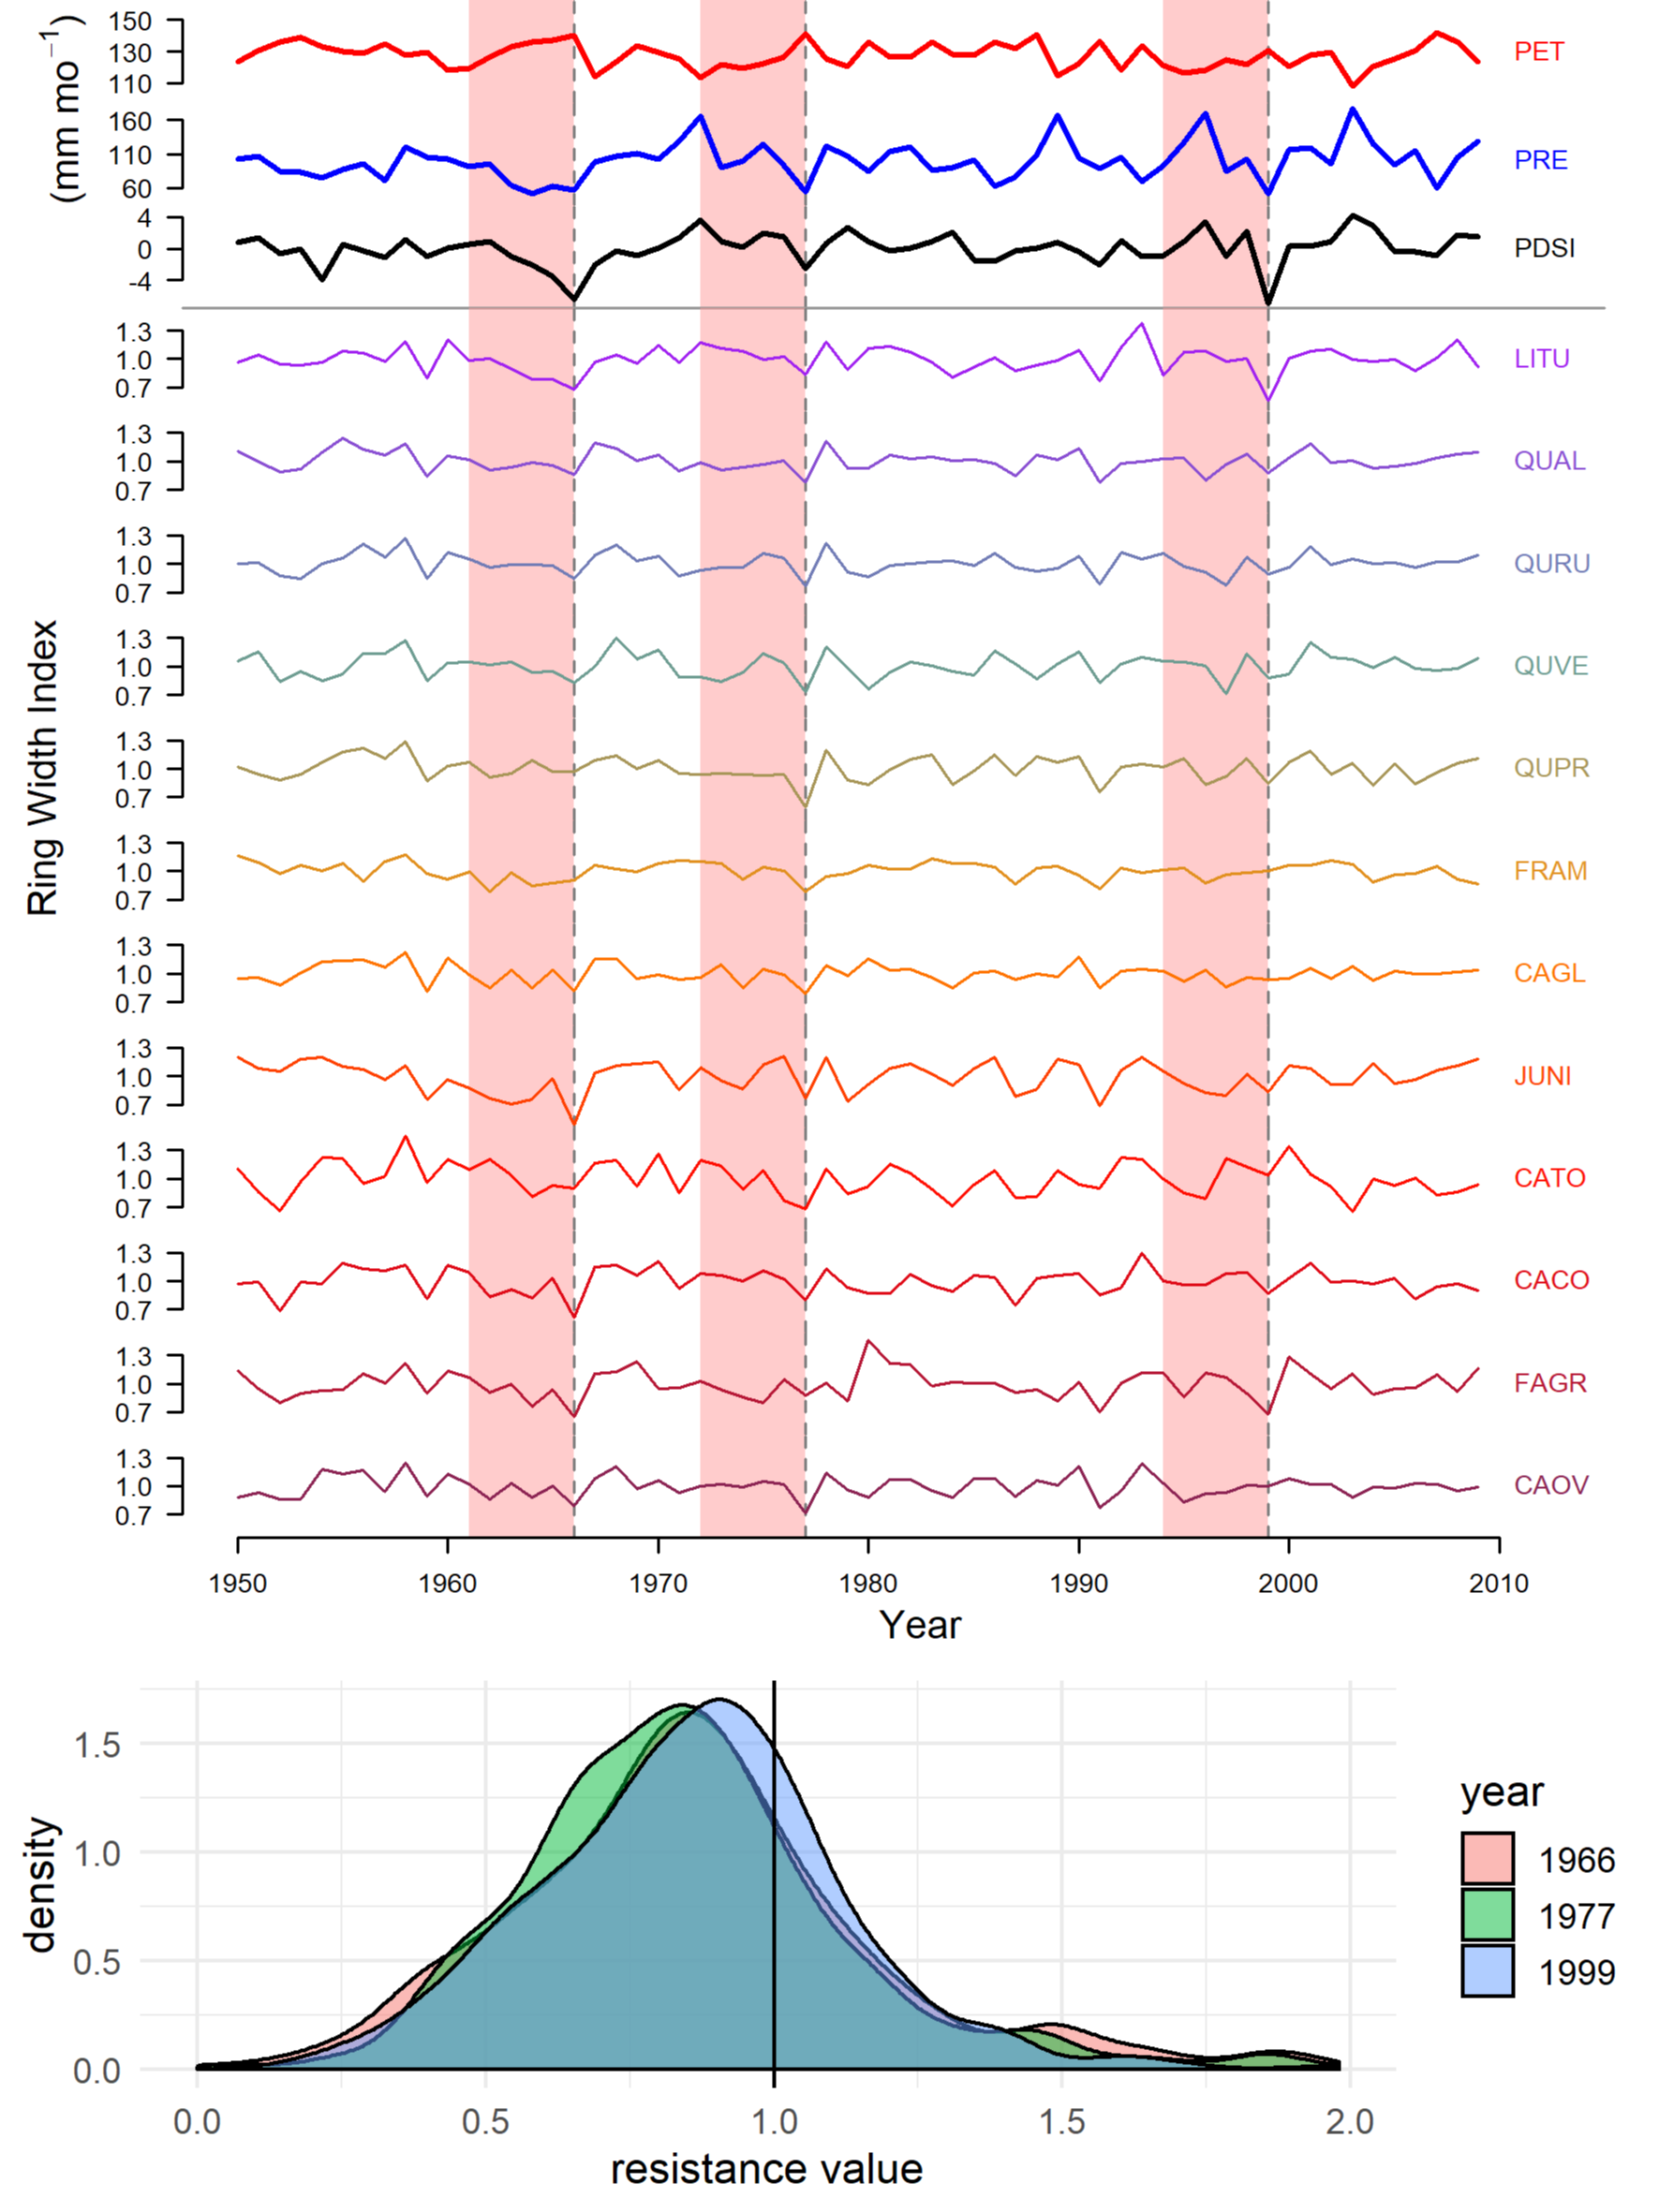
\includegraphics[width=5.20833in,height=\textheight]{tables_figures/Figure1.png}
\caption{\textbf{Figure 1. Climate and species-level growth responses
over our study period, highlighting the three focal drougths (a) and
community-wide responses} Time series plot (a) shows peak growing season
(May-August) climate conditions and residual chronologies for each
species. Focal droughts are indicated by dashed lines, and shading
indicates the pre-drought period used in calculations of the resistance
metric. Figure modified from Helcoski \emph{et al.} (2019). Density
plots (b) show the distribution of resistance values for each drought.}
\end{figure}

\begin{figure}
\centering
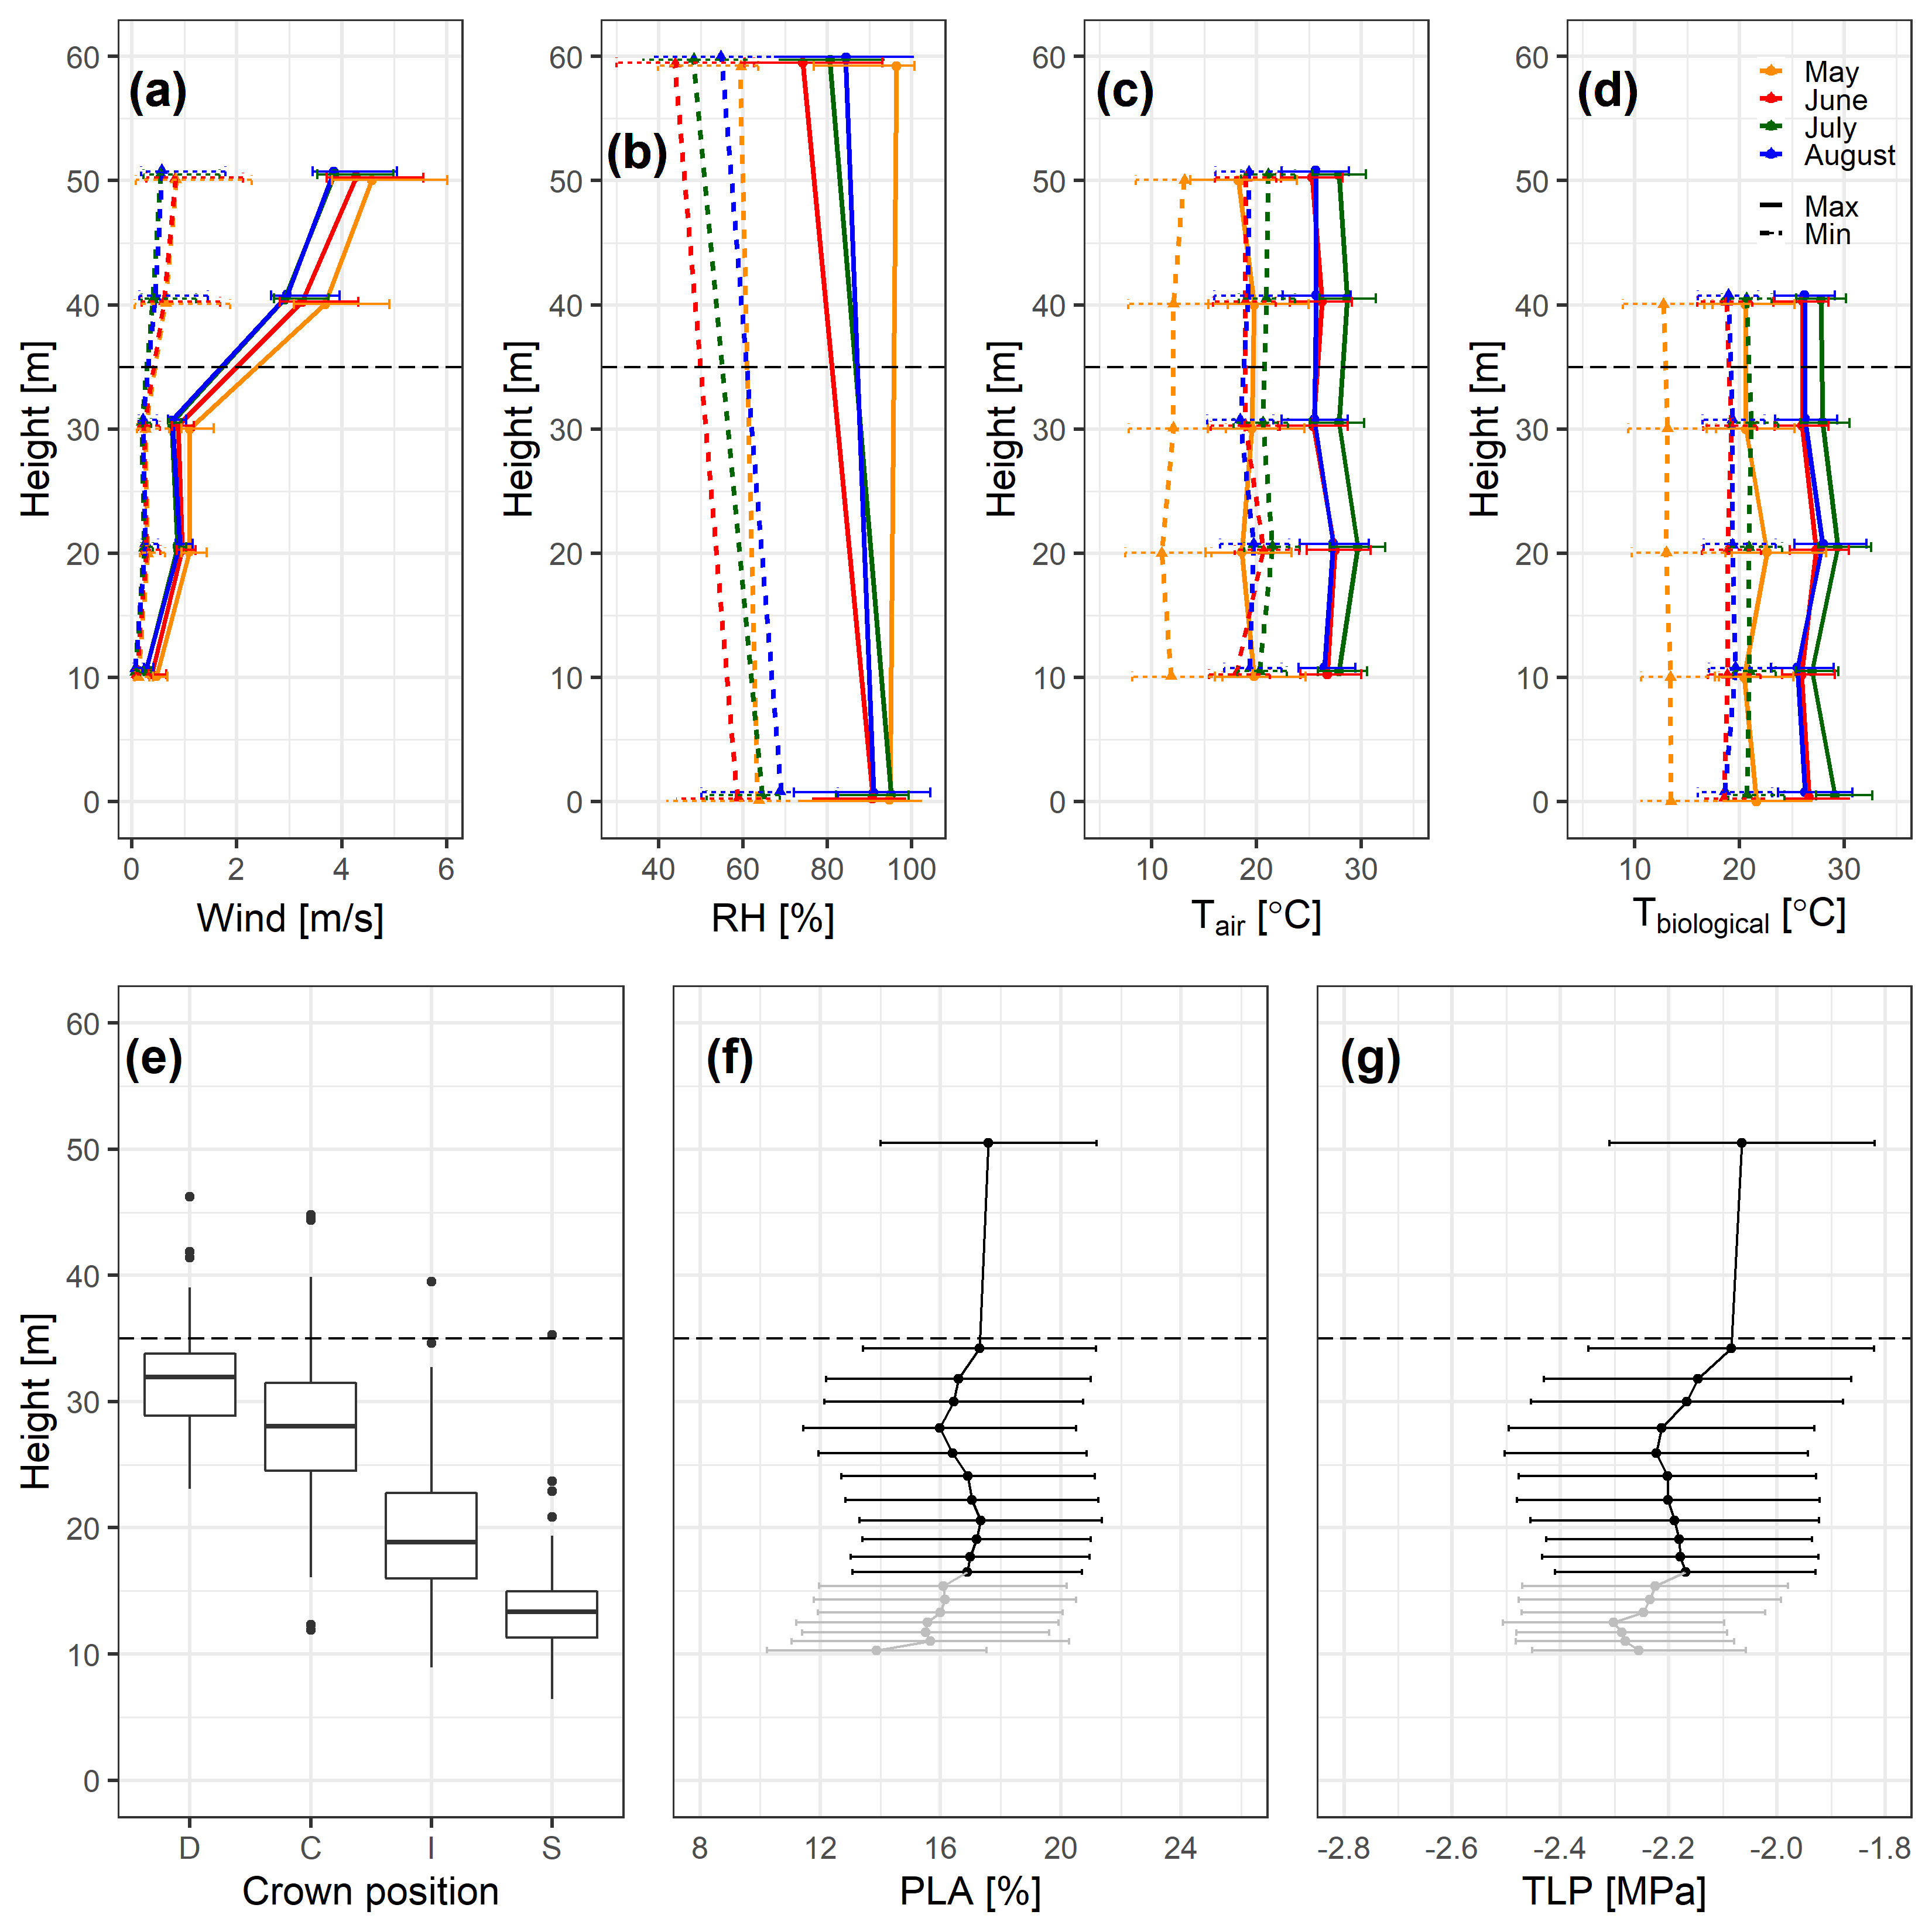
\includegraphics[width=5.20833in,height=\textheight]{tables_figures/Figure2.png}
\caption{\textbf{Figure 2. Height profiles in growing season climatic
conditions, tree heights by crown position, and leaf hydraulic traits}
The top row shows averages (\(\pm\) SD) of daily maxima and minima of
(a) wind speed, (b) relative humidity (\(RH\)), and (c) air temperature
(\(T_{air}\)) averaged over each month of the peak growing season
(May-August) from 2016-2018. In these plots, heights are slightly offset
for visualization purposes. Also shown are (d) 2018 tree heights by
canopy position (see Table 2 for codes) and vertical profiles in (e)
\(PLA_{dry}\) and (f) \(\pi_{tlp}\). In (e-f), values are community-wide
averages across height bins (plotted at upper end of height bin), with
grey indicating bins for which species-level trait measurements are
available for \textless75\% of individuals. In all plots, the dashed
horizontal line indicates the 95th percentile of tree heigts in the
ForestGEO plot.}
\end{figure}

  \bibliography{book.bib,packages.bib}

\end{document}
